% !TEX root=../august-boeckh-hauptdokument.tex

\chapter[Kondizionale Operatoren]{Konditionale Operatoren. Das sind Boole’sche Operatoren, die eine Menge Spaß machen}

\section{Widmung}
%\toggletrue{hund}
Diese Doktorarbeit widme ich von Herzen 
\iftoggle{hund}
{meinem Hund.}
{meinen lieben Eltern.}

%---
%  Folgendes Szenario: In der offiziellen Abgabeversion möchte ich meinen Eltern danken. 
%  Aber ein Extraexemplar soll meinem Hund gewidmet sein.
% Kann man das machen, dass man das irgendwie automatisch ändern kann?
%---


\section{Abbildungen}




\begin{figure}[h]
{\missingcopyright%muss in geschweifte Klammern gesetzt werden, da Schalter
\subcaptionbox%
{Alexander von Humboldt}%
{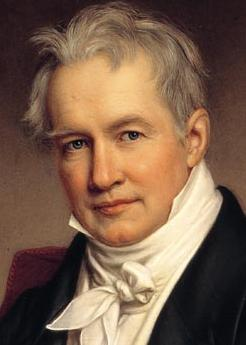
\includegraphics[
height=0.4\textwidth]{figures/alexander.jpg}}}
\hfill
\subcaptionbox{Wilhelm von Humboldt}{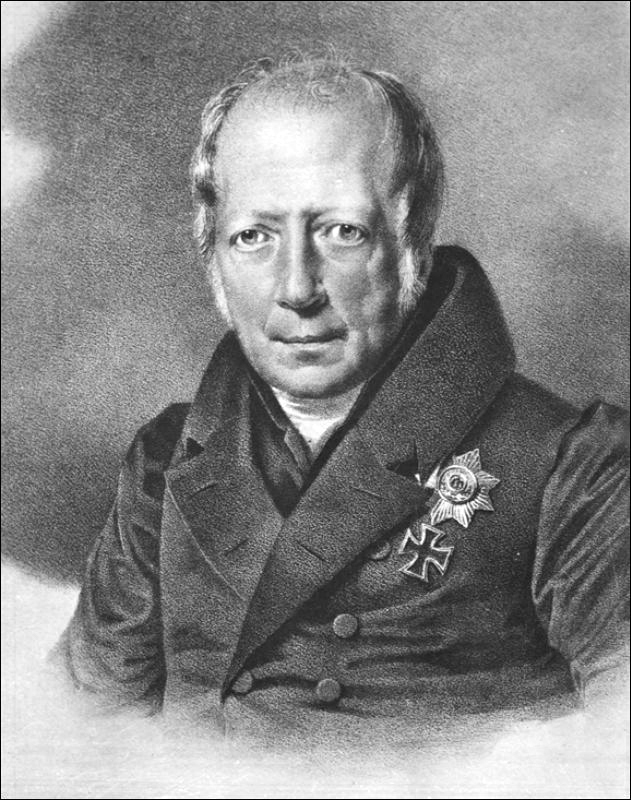
\includegraphics[height=0.4\textwidth]{figures/wilhelm.jpg}}
\label{fig:bruederhumboldt}
\caption{Die zwei Brüder von Humboldt}
\end{figure}



%--------------------------------
% Jetzt wird es schwierig: Die zwei Brüder sollen nebeneinander gesetzt werden.
% alexander.jpg und wilhelm.jpg
% Als Bildunterschrift: Alexander von Humboldt // Wilhelm von Humboldt
% Als gemeinsame  Bildunterschrift: Die Brüder von Humboldt
% Die Bilder bitte gleich hoch setzen.
%-------------------------------


%---
% Ich habe allerdings nur für Wilhelm die Druckgenehmigung bekommen,
% nicht für Alexander.
% Das heißt, dass in meiner Abgabeversion beide Bilder zusehen sein müssen,
% in der finalen Printfassung muss Alexander ausgeblendet werden.
% Die Maße und die Bildunterschrift sollen erhalten bleiben
% und nur das Bild mit einem Platzhaltertext versehen werden.
%---







